\documentclass[a4paper,12pt]{article}

\usepackage{fancyhdr}
\pagestyle{fancy}
\fancyhf{}
\fancyhead[R]{\thepage}

\usepackage{tikz}
\usetikzlibrary{shapes.gates.logic.US,trees,positioning,arrows}


\usepackage{amsfonts}
\usepackage{amsmath}
\usepackage{xcolor}
\usepackage{amssymb}
\usepackage[colorlinks]{hyperref}


\newcommand{\R}{\color{red}}
\newcommand{\G}{\color{green}}
\newcommand{\B}{\color{blue}}
\newcommand{\Gr}{\color{gray}}
\definecolor{orange}{HTML}{FF7F00}
\newcommand{\Or}{\color{orange}}


\newcommand{\V}{\vspace{2cm}}
%\newcommand{\P}{\pagebreak}


\newcommand{\A}{ \author{\it\Gr Md. Nirab Hossain}}
\newcommand{\C}{\title}
\newcommand{\D}{\date{August 9, 2019} \maketitle}

\begin{document}
	\C{\bf\B\Huge A Short Note On Cryptography} \A \D
	\pagebreak
	\section{\Large Chapter 1\\\\}
	\begin{center}
		{\Huge\sc\Or Background}
	\end{center}
\vspace{8cm}
	\subsection{Definitions}
	{\bf Cryptography:}
	It is the process of secrecy that makes data unreadable. The main purpose is the information to be kept secret or sent secretly by encoding to the receiver and then decode it. That is, cryptography makes information unusable for un authorized user. It encrypts the data into unreadable format and sends it to the receiver who can decode it back to the readable format and use the information.\\
	In a word, cryptography attempts to a secure communication. It includes two main processes. 
	\begin{enumerate}
		\item {\bf Encryption:} It allows the data to convert into an unreadable format. It involves some codes that encrypts the data which can be sent anywhere safely. Because none reads it without key.\\
		{\it The key} is nothing but a set of information to break encryption code.
		
		\item {\bf Decryption:} It allows the unreadable data to decode into the original text format with a key. One who has key is assumed to be an {\it authorized user}. Only authorized users have legal access to the {\it ciphertexts.} {\it A ciphertext or cyphertext} is the result of encryption performed on plaintext using an algorithm and that algorithm is called {\it cipher}.
	\end{enumerate}

\V
	\subsection{Kerckhoffs' Principle of Keys}
	We have discussed previously why the key is important. Significance of key depends on the strength of cipher. The lower the cipher strength, the lower the security. Anyone can have the key i.e. break the code if the code is not so strong.
	
	\noindent The Netherlands born cryptographer {\B Auguste Kerckhoffs} stated six principles of practical cipher design in his journal in 1983 named {\it le Journal des Sciences Militaires}. One of the six is widely known as Kerckhoffs' principal. We only need to describe that statement to observe the significance of key. This can be stated as: 
	\begin{center}\it A cryptosystem should be secure even if everything \\about the system, except the key, is public knowledge.\end{center}	
	\noindent That is, the cipher may be strong but it must not be kept secret but the key should contain the necessary secure information only. There is two main reasons behind this statement.
	\begin{enumerate}
		\item It is more convenient to share a key (about 100-200bit say) than an algorithm. The key is just a string. But the code is an application containing a huge size. So, it has a good chance of being leaked.
		
		\item The Replacement of key is very much easier compared to the replacement of whole algorithm. Once one knows the algorithm, then nothing happens if the key is not in his hand. On the other hand, the key is easily replaceable once key is in enemy's hand.
	\end{enumerate}
	The {\B Shannon's} Maxim: 
	\begin{center}\it Enemy knows the system\end{center} 
is just the reformulation of {\B Kerckhoffs'} principle.
\V
	\subsection{Working Area of Cryptography}
	There are two main areas of cryptography to talk about. They are {\it cryptographic   algorithm and protocols} and {\it network and internet security.\\\\}
	{\bf Network Security and protocols:}This part consists of four parts:
	\begin{enumerate}
		\item {\bf Public Key Encryption:} One key is used for both encryption and decryption. Transformation of key is significant here. This key must be kept secret. This key is also known as {\it Symmetric key}.
		
		\item {\bf Private Key Encryption:} The encryption and decryption keys can be made different(but not necessary). The keys are interchangeable. But in case both keys are known for sender and receiver previously and same keys are used repeatedly, the key transfer is not that important. This key is also known as {\it Asymmetric key}, since a pair distinct of keys is created. If one is made public, the other is protected. Which is why the key is public type. Google form is an example of this.
		
		\item {\bf Data Integrity Algorithm:} Used to protect information such as documents from alteration.
		
		\item {\bf Authentication Protocols:} This relates with authenticity of both information and user.
	\end{enumerate}
{\bf Network and internet security:}This is a huge topic consisting of measures to deter, prevent,
detect, and correct security violations that involve the transmission of information.\\\\
\noindent The discussion can be picturised as following:
\begin{center}		
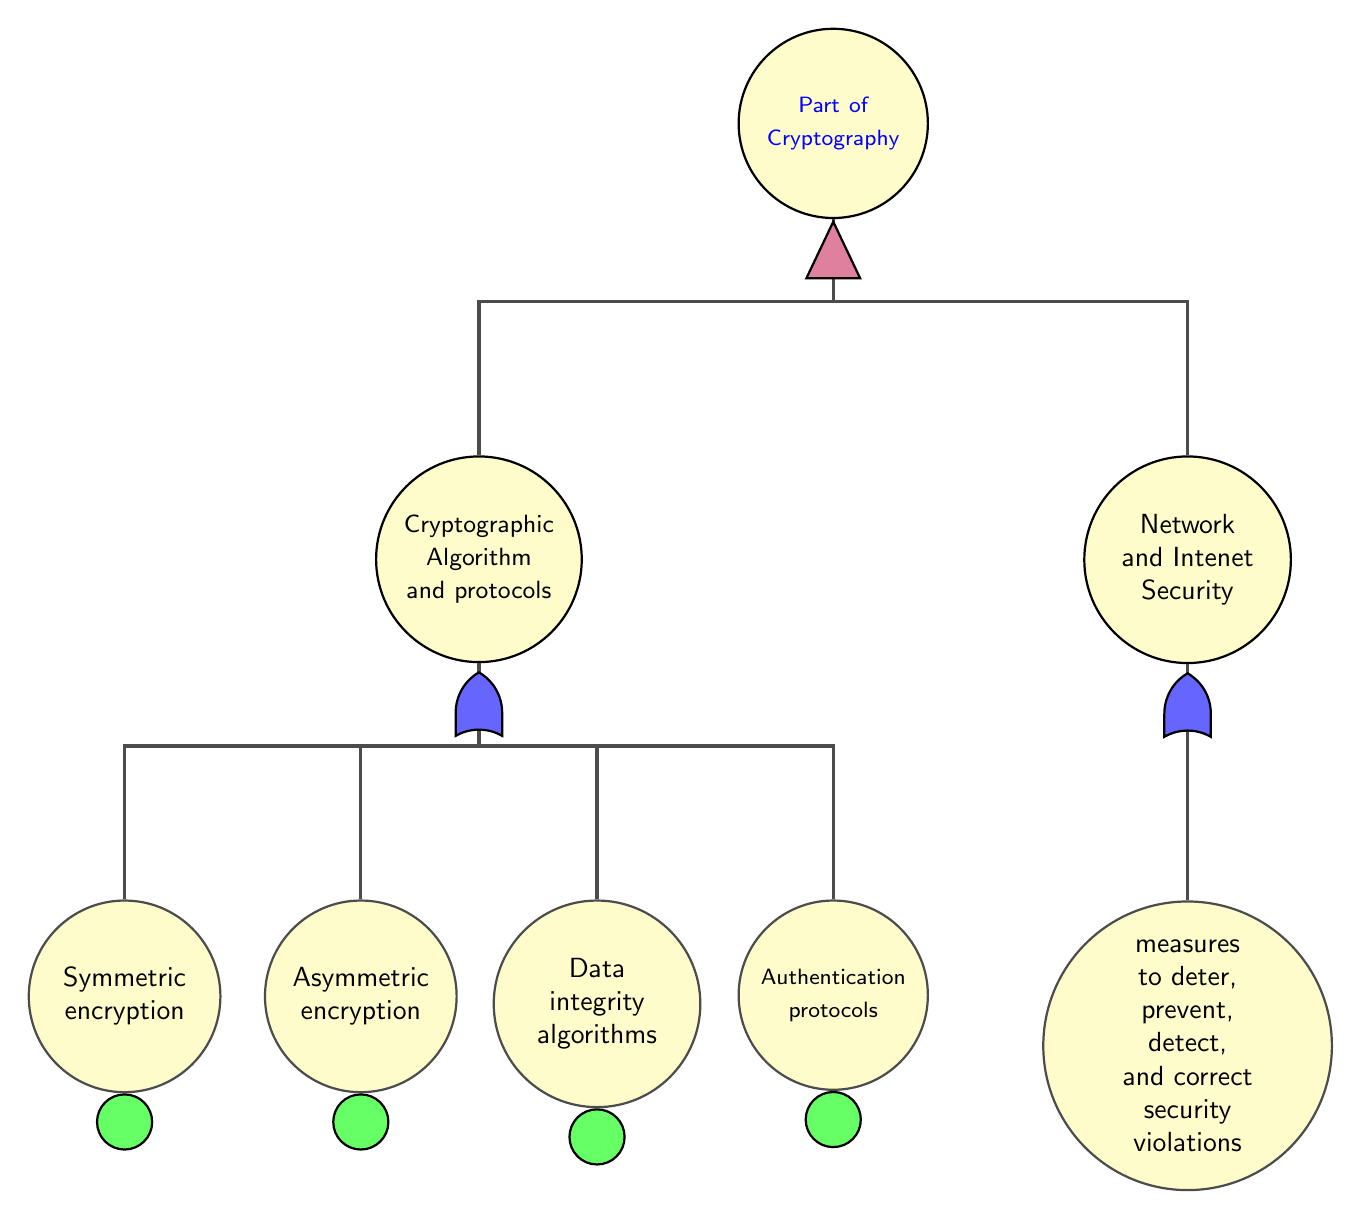
\begin{tikzpicture}[
% Gates and symbols style
and/.style={and gate US,thick,draw,fill=red!60,rotate=90,
	anchor=east,xshift=-1mm},
or/.style={or gate US,thick,draw,fill=blue!60,rotate=90,
	anchor=east,xshift=-1mm},
be/.style={circle,thick,draw,fill=green!60,anchor=north,
	minimum width=0.7cm},
tr/.style={buffer gate US,thick,draw,fill=purple!50,rotate=90,
	anchor=east,minimum width=0.8cm},
% Label style
label distance=3mm,
every label/.style={blue},
% Event style
event/.style={circle,thick,draw,fill=yellow!20,text width=2cm,
	text centered,font=\sffamily,anchor=north},
% Children and edges style
edge from parent/.style={very thick,draw=black!70},
edge from parent path={(\tikzparentnode.south) -- ++(0,-1.05cm)
	-| (\tikzchildnode.north)},
level 1/.style={sibling distance=9cm,level distance=3cm,
	growth parent anchor=south,nodes=event},
level 2/.style={sibling distance=3cm},
%%  For compatability with PGF CVS add the absolute option:
%   absolute
]
%% Draw events and edges
\node (g1) [event] {\B\footnotesize Part of Cryptography}
child{node (a1) {\small Cryptographic Algorithm and protocols}
	child {node (b11) {Symmetric encryption}}
	child {node (b12) {Asymmetric encryption}}
	child {node (b13) {Data integrity algorithms}}
	child {node (b14) {\footnotesize Authentication protocols}}
}
child{node (a2) {Network and Intenet Security}
	child {node(b21){measures to deter, prevent,
			detect, and correct security violations}}
}
;
\node [tr]	at ( g1.south){};
\node [or]	at ( a1.south){};
\node [or]	at (a2.south){};
\node [be]	at (b11.south){};
\node [be]	at (b12.south){};
\node [be]	at (b13.south){};
\node [be]	at (b14.south){};

\end{tikzpicture}
\tt The block diagram of Cryptographic area
\end{center}
\V
	\subsection{Computer security and the CIA triad}
	The definition of computer security was given by NIST({\it National Security of Standard and Technology}). The definition is as follows:
	\begin{center}
		\it The protection afforded to an automated information system
		in order to attain the applicable objectives of preserving the integrity, availability,and confidentiality of information system resources (includes hardware, software,firmware, information/data, and telecommunications).
	\end{center}
\noindent Here, three terms are introduced of great importance. These are confidentiality, integrity and availability which are together called the { \bf {\it CIA triad}}.
 {\R \\\\There will be an image right here.} 
\begin{itemize}
	\item {\bf Confidentiality:} The term refers to the information keeping confidential from the unauthorized users and disclosing to the authorized users.
	\item {\bf Integrity:} It refers to control the addition, destruction and editing or modifying of information. So, hacking is a loss of integrity of security.
	\item {\bf Availability:} This relates with easy access of information to the authorized users. It is very important, because users may not prefer any algorithm that is hard to understand or run.
\end{itemize}


	\subsection{Security Attack}
	Security attack of computer can be classified based on various things, like harmfulness, attacking strategy etc.
	In terms of harmfulness, security attack can be classified as active and passive attacks:
	\begin{itemize}
		\item {\bf Passive attack:} Attacker takes knowledge form the system but doesn't harms the computer.
		\item {\bf Active attacks:}Here unauthorized user alters or attempts to alter the system which affects the computer.\\
	\end{itemize}
	Security attack is classified into four following part in terms of strategy:
	\begin{itemize}
		\item {\bf Ciphertext only attack:}In this attack, ciphertext is observed to determine plaintext.
		\item {\bf Known plaintext attack:} Here, the enemy some portion of
			ciphertexts or plain texts that are encrypted with the similar key. Then, approaching with the information is known plaintext attack.
		\item {\bf Chosen plaintext attack:} This process involves random plaintext to encrypt and generate ciphertext to get the desired ciphertext. 
		\item {\bf Chosen ciphertext attack:} This is the reverse process of {\it chosen plaintext attack.} In this attack, adversary approaches to get plaintext by assuming ciphertext.
		
		{\R There will be name of reference books}
		
	\end{itemize}
	\section{\Large CHAPTER 2}
	\begin{center}{\Huge\Or\sc AES}\end{center}
	\subsection{History}
			Write description here
\end{document}
